\section{Results}
\label{sec:results}

This section presents the result of the algorithm for the different worlds we introduced in the previous section. We are examining the algorithm using different heuristic strategies to measure their impact. We use four different strategies: using both heuristics, using only NN-heuristic, using only the Machine-heuristic, and using no heuristic.

\subsection{Manually Created Worlds}

For the first manually created world, we get the optimal solution (13 steps) for every strategy. It is the expected result given that there is just one petition and one machine. Figure \ref{fig:t1} shows that both the optimal solution (green line) and the strategy using both heuristics (red line) compute the same result.

\begin{figure}[!hbt]
  \centering
  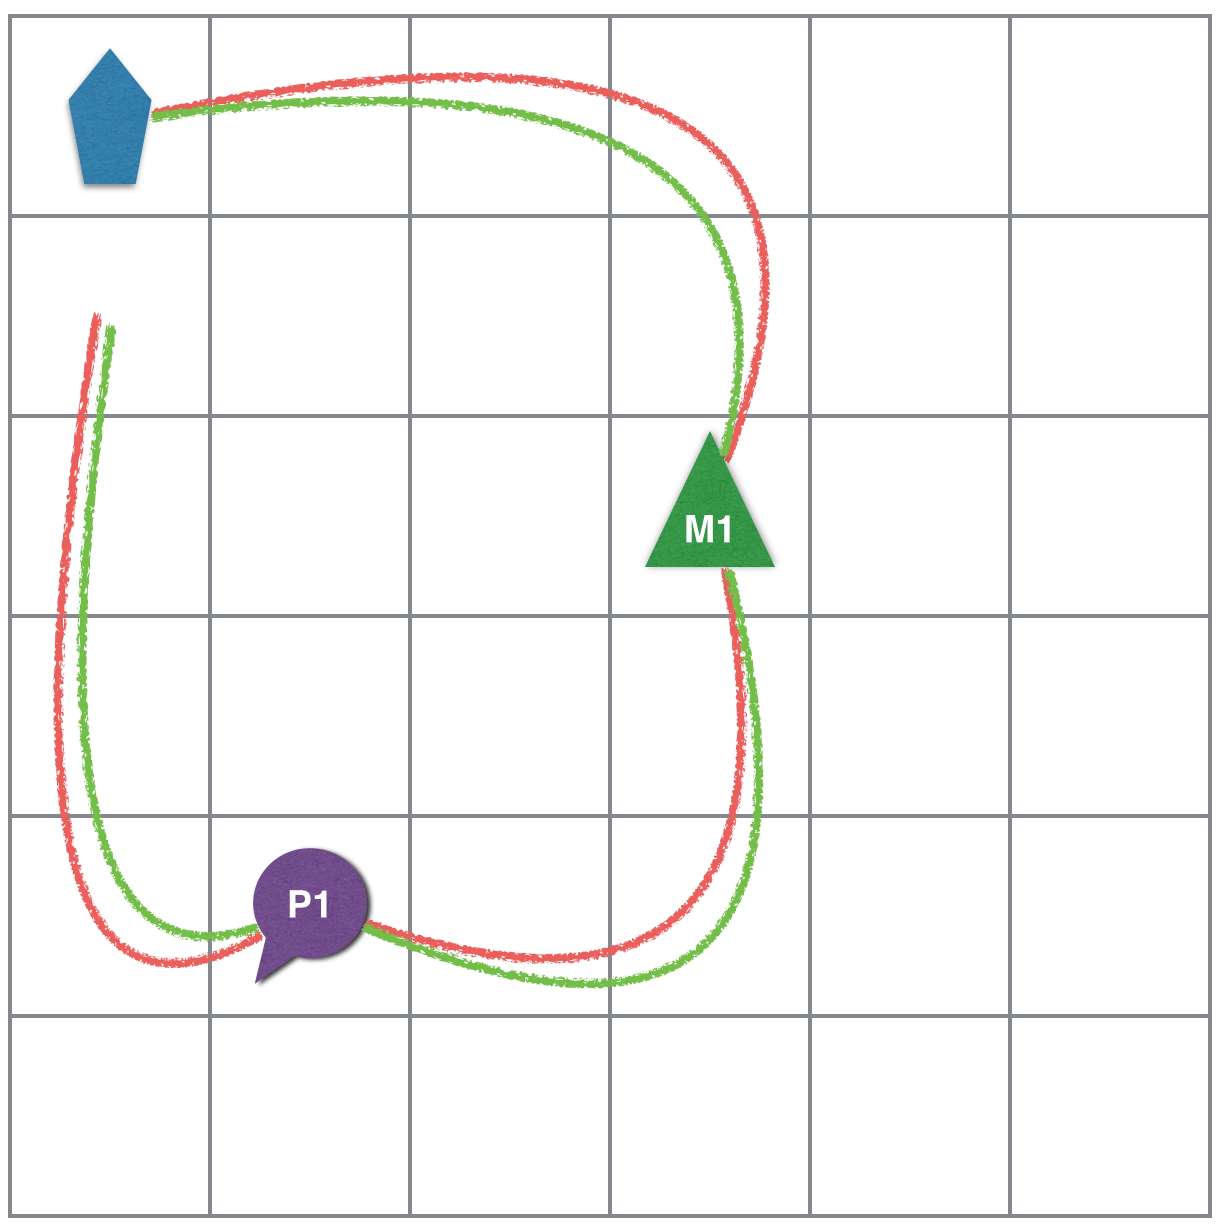
\includegraphics[width=0.5\textwidth]{img/t1}
  \caption{Results for first manually created example}
  \label{fig:t1}
\end{figure}

For the second example, the Machine-heuristic alone gives us the optimal solution (9 steps), no matter how the petitions to be served are ordered at the beginning, since there is only one petition. Without the Machine-heuristic, the machine M1 is chosen, resulting in 13 steps. Figure \ref{fig:t2} shows that both the optimal solution and the heuristic solution are the same.

\begin{figure}[!hbt]
  \centering
  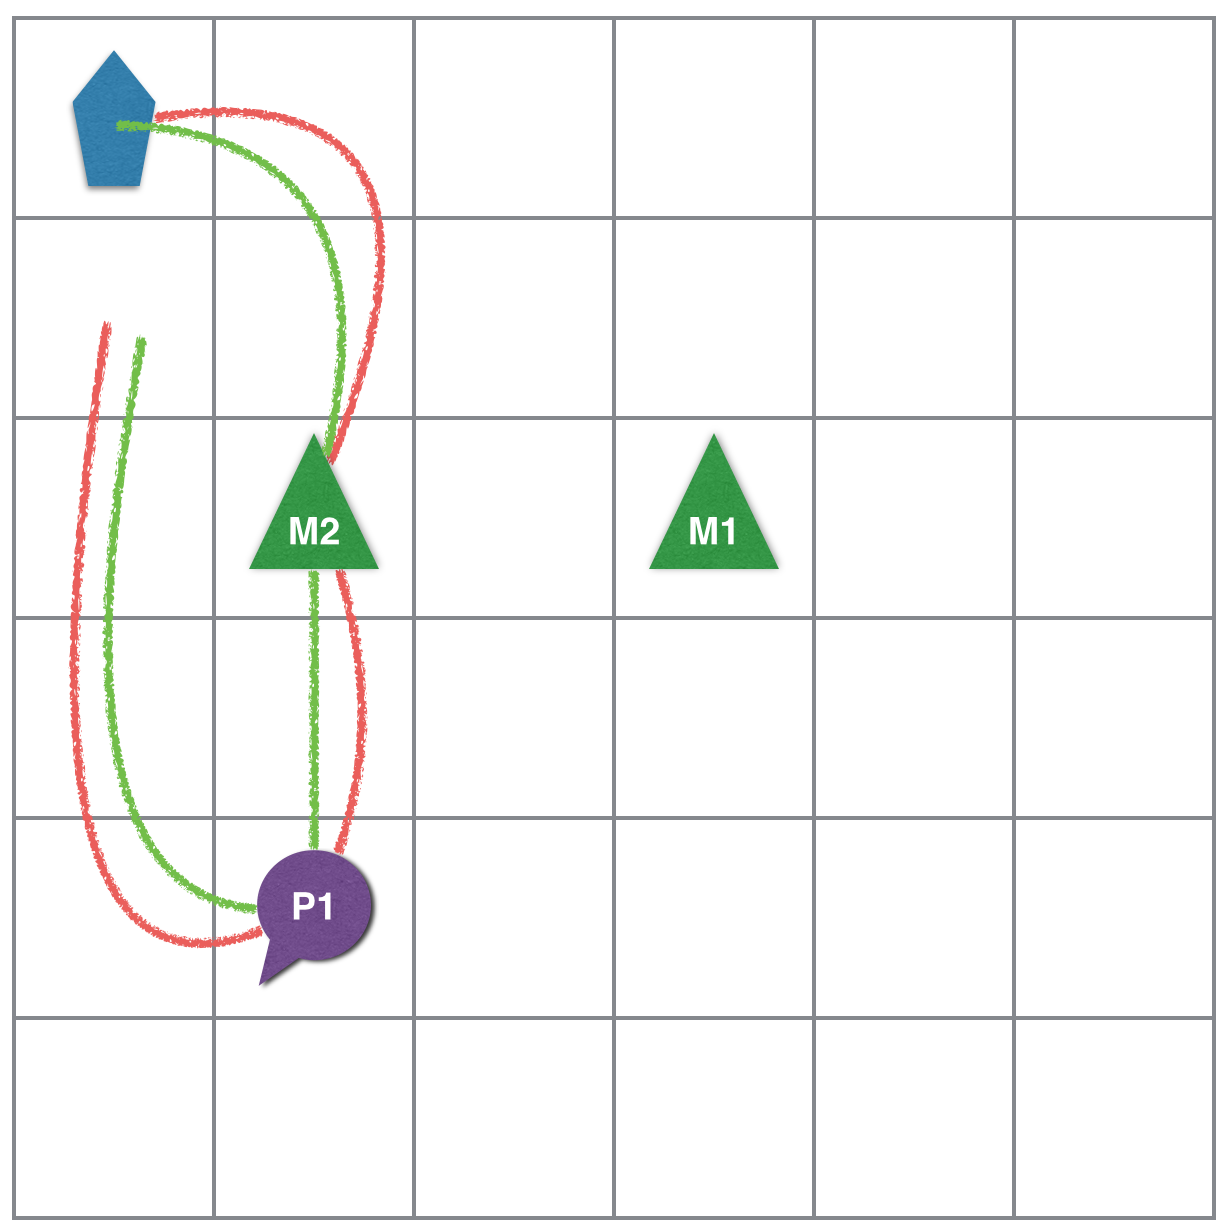
\includegraphics[width=0.5\textwidth]{img/t2}
  \caption{Results for second manually created example}
  \label{fig:t2}
\end{figure}

For the third example, even using both heuristics, the algorithm is not able to get the optimal solution of 27 steps. The NN-heuristic does not choose the optimal order of petitions, leading to a sub-optimal solution of 29 steps. This solution is still relatively close to the optimal one. When only using the NN-heuristic, the results are considerably worse with 45 steps. Figure \ref{fig:t3} shows how the optimal and the heuristic plan diverge after serving $P3$ since the NN-heuristic came up with a different ordering of petitions ([$P1, P3, P4, P2$] instead of [$P1, P3, P2, P4$]).

\begin{figure}[!hbt]
  \centering
  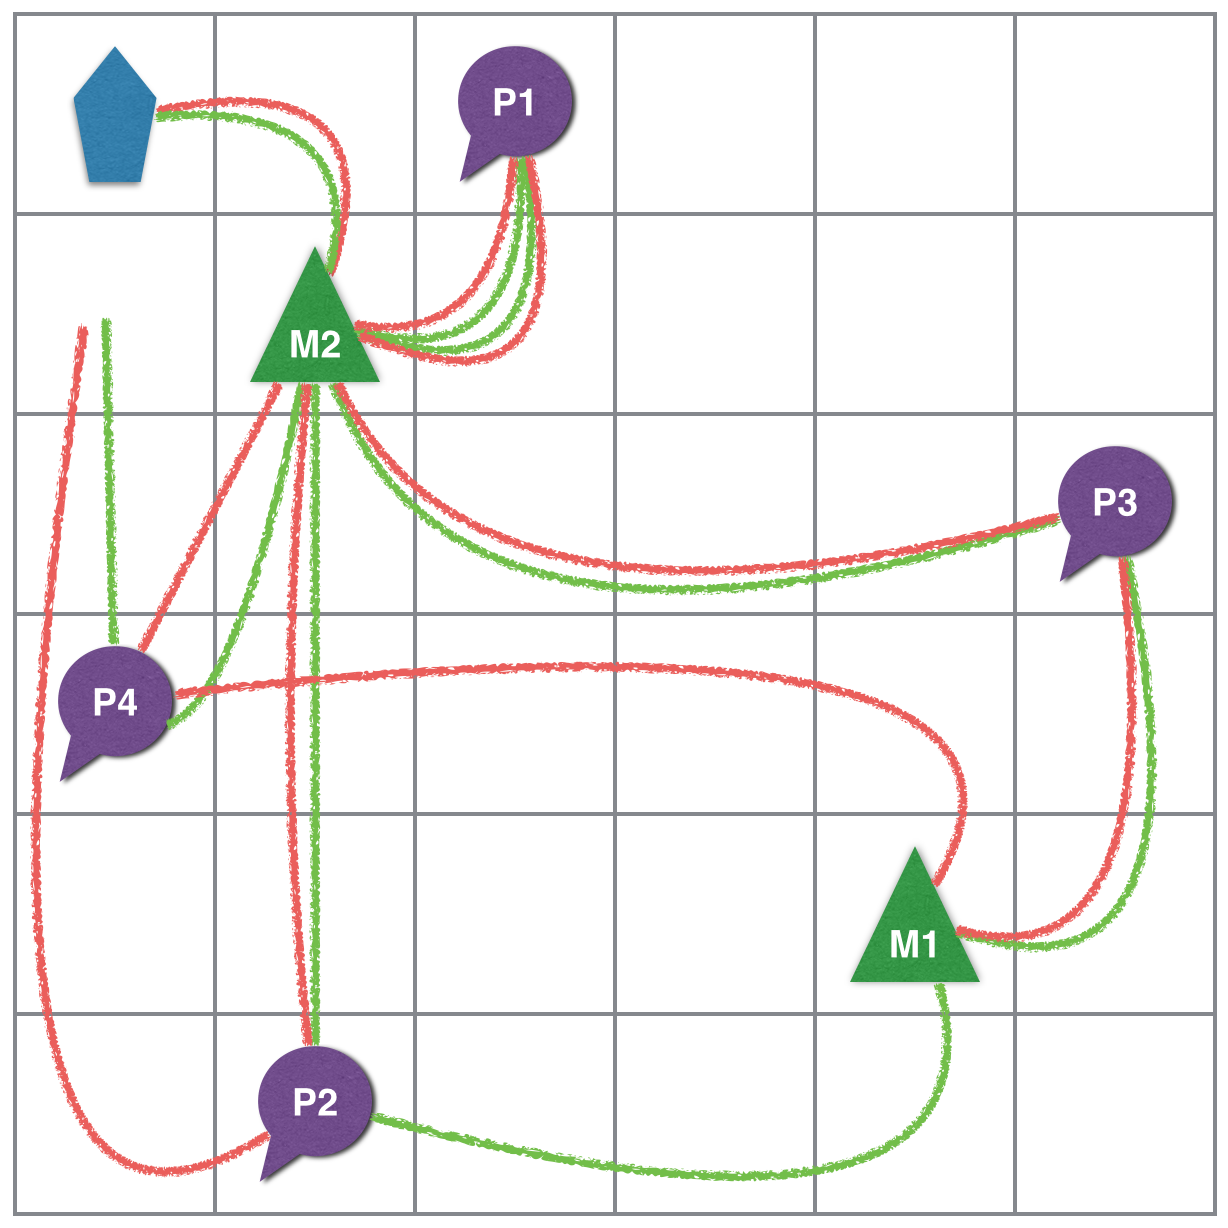
\includegraphics[width=0.5\textwidth]{img/t3}
  \caption{Results for third manually created example}
  \label{fig:t3}
\end{figure}

\subsection{Automatically created worlds}

Figure \ref{fig:abc1} shows the average result (blue dot) and standard deviation (blue bar) of the step error for different heuristics. The step error is defined as the $\Delta$ between the steps that the planner came up with and the steps of the optimal solution.

NN-TS means, that the NN-heuristic was used to determine the order of petitions. Random means, that a random order of petitions was used. Closest-M means, that the Machine predicate heuristic was used, while First M corresponds to simply picking the first Machine predicate in the list.


\begin{figure}[!hbt]
  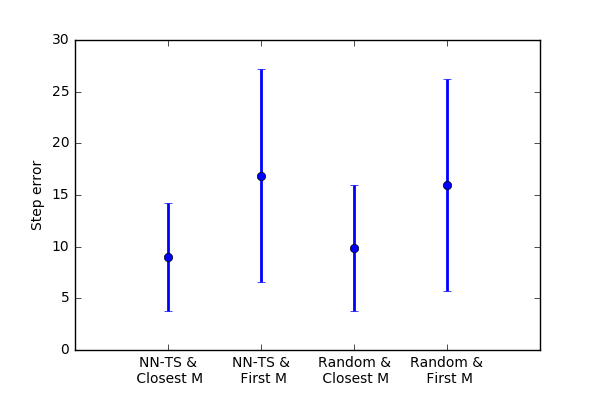
\includegraphics[width=1\textwidth]{img/step_error_vs_heuristic}
  \caption{Step Errors for Different Heuristic}
  \label{fig:abc1}
\end{figure}

As we can see in figure \ref{fig:abc1}, using both heuristics yields the best results on average. Not using the NN-heuristics only worsens the results slightly. Deactivating the Machine-heuristic makes the step error increase dramatically - hence it has the highest impact on success.

Figure \ref{fig:abc2} shows how often the different heuristic configuration yielded the smallest step error. Again we can see, that using both heuristics yields the best results with a winner ratio of more than 0.6. This means that in 60\% of the cases, using both heuristics yielded the best result. The values don't add up to 1.0 because sometimes several strategies had the same result.

\begin{figure}[!hbt]
  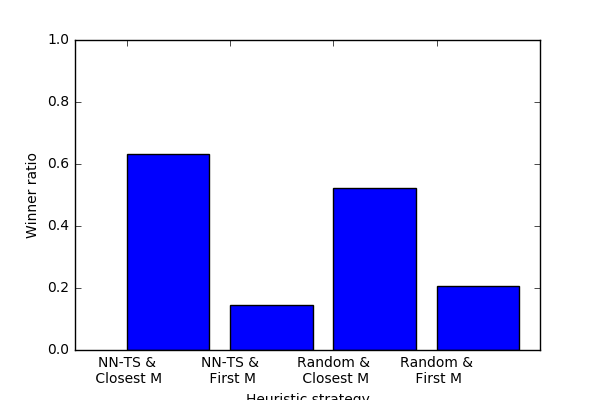
\includegraphics[width=1\textwidth]{img/winner_ratio_vs_heuristic}
  \caption{Ratio of Best Solution for Different Heuristic}
  \label{fig:abc2}
\end{figure}

Figure \ref{fig:abc3} shows the relationship between the complexity of the world measured in numbers of petitions and the average step error. As we can see, for increasing the complexity, using both heuristics yields increasingly better results compared to the other strategies. For high numbers of petitions it becomes increasingly important using the NN-heuristic to get good results.

\begin{figure}[!hbt]
  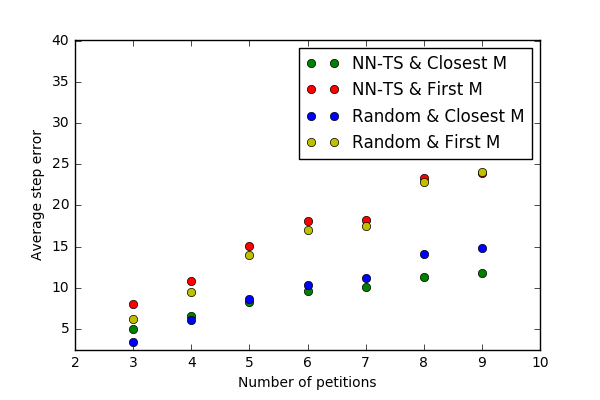
\includegraphics[width=1\textwidth]{img/avg_error_vs_petitions}
  \caption{Average Result and Petition Complexity}
  \label{fig:abc3}
\end{figure}

Figure \ref{fig:abc4} shows the relationship between the complexity of the world measured in numbers of machines and the average step error. There is less correlation between machine complexity and the step error, than we observed with the petition complexity. For high numbers of machines the importance of using the Machine-heuristic increases, since it can find much better results than picking an arbitrary machine. 

\begin{figure}[!hbt]
  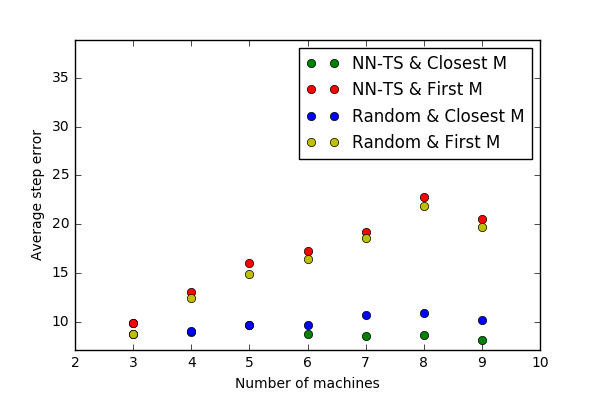
\includegraphics[width=1\textwidth]{img/avg_error_vs_machines}
  \caption{Average Result and Machine Complexity}
  \label{fig:abc4}
\end{figure}

